\documentclass{beamer}

\usetheme{Warsaw}

\title{EE1390}
\subtitle{MATRIX PROJECT}
\author{EE18BTECH11003 , EE18BTECH11013}
\date{}
\usepackage{amsmath}
\usepackage{graphicx}

\begin{document}





\begin{frame}
\titlepage
\end{frame}
\begin{frame}{Question-6}
Q. The sides of a rhombus is parallel to the lines
     (1 -1)X+2=0,
     (7 -1)X+3=0.
   If the diagonals of a rhombus intersect at 
     P(1,2)
   and the vertex C (different) from the origin is
   on the y-axis, then find the ordinate of ! C.
\end{frame}

\begin{frame}{Solution}
Given two lines are parallel to the sides of rhombus.\\
(1 -1)X+2=0 \\ (7 -1)X+3=0\\
The intersection point of diagonal P is
\section{matrices}
\[
P=\begin{pmatrix}
1\\
2
\end{pmatrix}
\]
where 
\[
X=\begin{pmatrix}
x \\
y
\end{pmatrix}
\]
Let 
\[
A=\begin{pmatrix}
0\\
a
\end{pmatrix}
\]
Now from above two equations let say slopes are m1 and m2
where m1=1 and m2=7 
\end{frame}
\begin{frame}
Now the angle between the given lines(sides of rhombus) containing diagonal other the diagonal containing C is 
 $tan\theta =(m2-m1)/(1+m1*m2)$\\
 $tan\theta =(7-1)/(1+7)$\\
 $tan\theta =3/4$\\
 $\theta =36.87 degree$\\
 Now the angle between diagonal and one of those lines is $\theta/2=18.435 degree$\\
 and $tan(\theta/2)=0.33$\\
 $tan(\theta/2)=(1-m)/(1+m)$\\
 0.33=(1-m)/(1+m) ;m=slope of diagonal other tha passing through A.\\
 after solving the equation we get m=1/2.
\end{frame}
\begin{frame}
Now the slope of the other diagonal is m=-2.\\
(diagonals are perpendicular to each other).\\
The equation of other diagonal is which is passing through (1,2)and slope is -2 is given as \\
 (2 1)X-4=0.\\
\section{matrix}
After puting X=C in above equation of diagonal we get
\[
A= \begin{pmatrix}
0\\
4
\end{pmatrix}
\]
That is the ordinate of C is 4.


\end{frame}


\begin{frame}
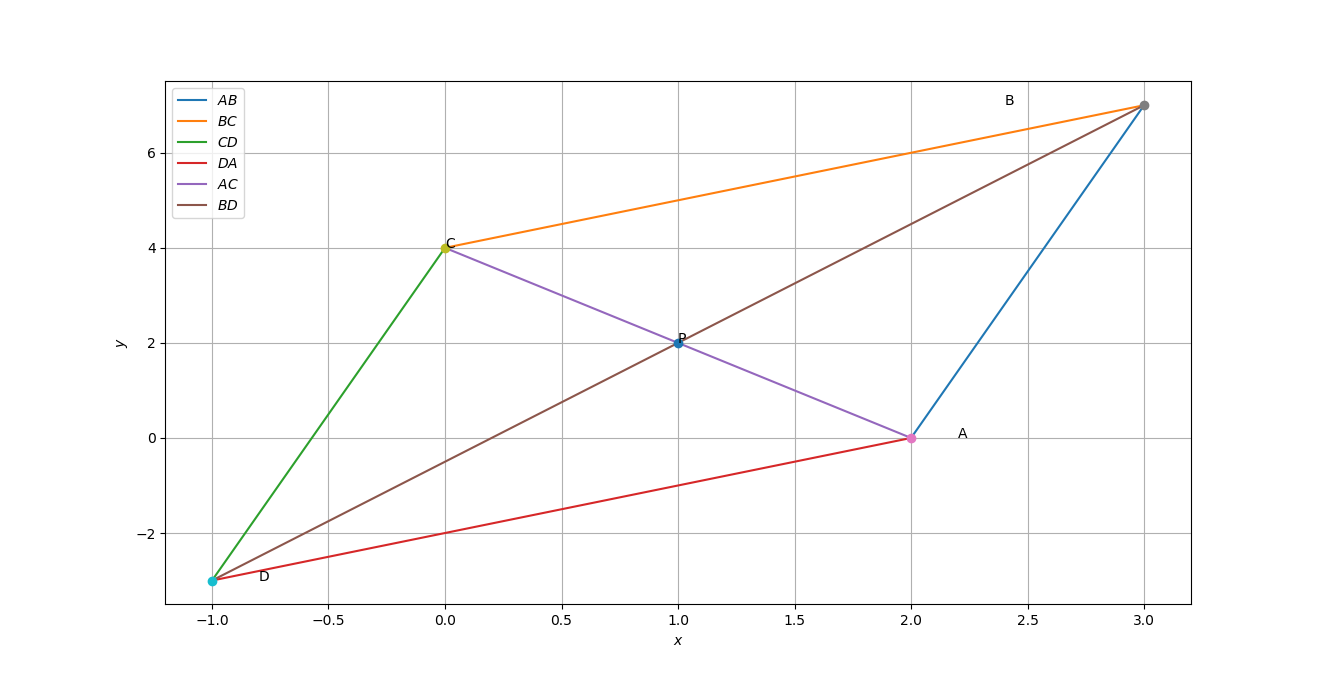
\includegraphics[scale=0.3]{Figure_1.png} 

\end{frame}


\end{document}